\documentclass[11pt,letterpaper]{book}
%-------------------paquetes
\usepackage{graphicx}
\usepackage[spanish]{babel}
\usepackage{listings}

\usepackage{color}

\definecolor{mygreen}{rgb}{0,0.6,0}
\definecolor{mygray}{rgb}{0.5,0.5,0.5}
\definecolor{mymauve}{rgb}{0.58,0,0.82}

\lstset{ 
	backgroundcolor=\color{white},   % choose the background color; you must add \usepackage{color} or \usepackage{xcolor}; should come as last argument
	basicstyle=\footnotesize,        % the size of the fonts that are used for the code
	breakatwhitespace=false,         % sets if automatic breaks should only happen at whitespace
	breaklines=true,                 % sets automatic line breaking
	captionpos=b,                    % sets the caption-position to bottom
	commentstyle=\color{mygreen},    % comment style
	deletekeywords={...},            % if you want to delete keywords from the given language
	escapeinside={\%*}{*)},          % if you want to add LaTeX within your code
	extendedchars=true,              % lets you use non-ASCII characters; for 8-bits encodings only, does not work with UTF-8
	firstnumber=1000,                % start line enumeration with line 1000
	frame=single,	                   % adds a frame around the code
	keepspaces=true,                 % keeps spaces in text, useful for keeping indentation of code (possibly needs columns=flexible)
	keywordstyle=\color{blue},       % keyword style
	language=Java,                 % the language of the code
	morekeywords={*,...},            % if you want to add more keywords to the set
	numbers=left,                    % where to put the line-numbers; possible values are (none, left, right)
	numbersep=5pt,                   % how far the line-numbers are from the code
	numberstyle=\tiny\color{mygray}, % the style that is used for the line-numbers
	rulecolor=\color{black},         % if not set, the frame-color may be changed on line-breaks within not-black text (e.g. comments (green here))
	showspaces=false,                % show spaces everywhere adding particular underscores; it overrides 'showstringspaces'
	showstringspaces=false,          % underline spaces within strings only
	showtabs=false,                  % show tabs within strings adding particular underscores
	stepnumber=2,                    % the step between two line-numbers. If it's 1, each line will be numbered
	stringstyle=\color{mymauve},     % string literal style
	tabsize=2,	                   % sets default tabsize to 2 spaces
	title=\lstname                   % show the filename of files included with \lstinputlisting; also try caption instead of title
}
%-------------------portada
\title{ARQUITECTURA EMPRESARIAL}
\author{Sandro bolaños}
%-------------------libro
\begin{document}
\maketitle
\tableofcontents
\listoffigures

\part{PROYECTO}
\chapter{Generalidades}
\chapter{Metodología}

\part{ARQUITECTURA}
\chapter{ADM-Archimate}
\section{Introducción}
contenido...
\newpage

\section{ADM}
contenido...

\begin{figure}[h!]
	\centering
	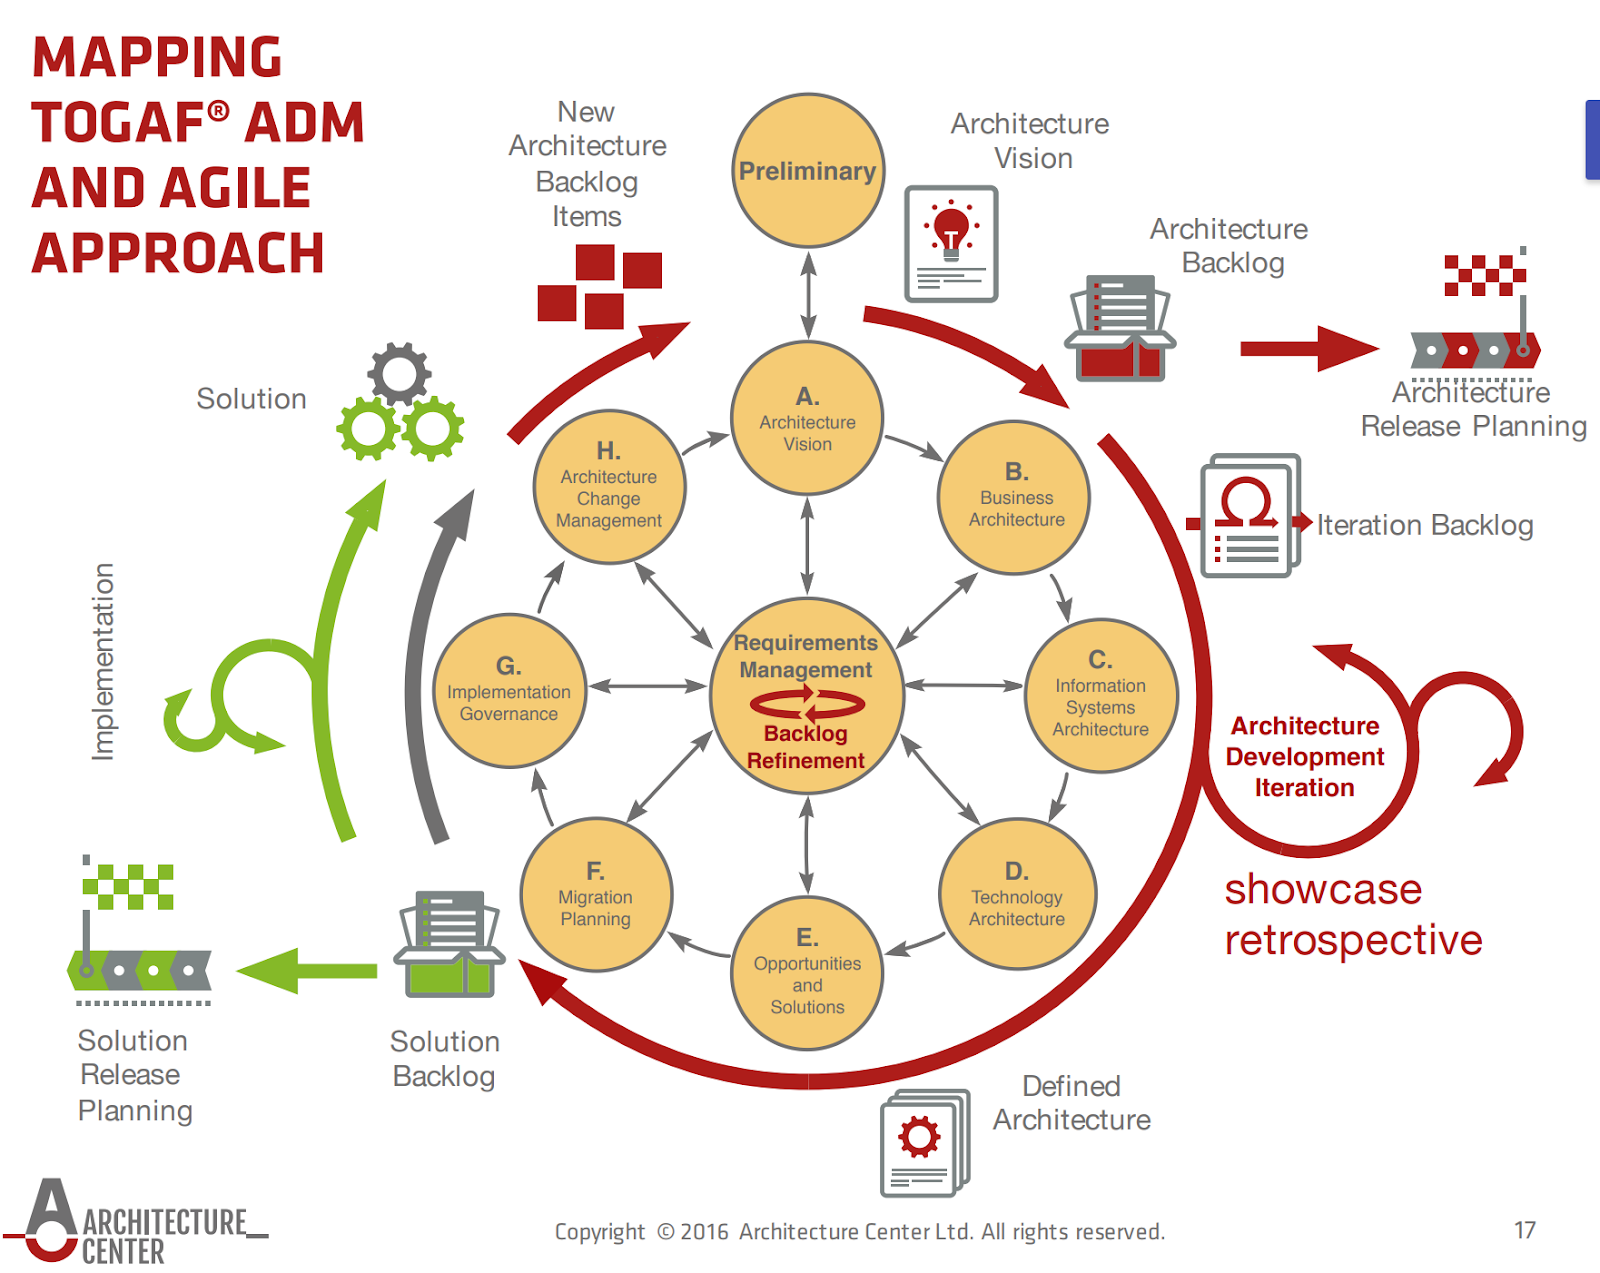
\includegraphics[width=0.7\linewidth]{ARQUITECTURA/imgs/adm}
	\caption{ADM \cite{SB,1579133,6337726,6337730,6827125}}
\end{figure}


\newpage

\section{Archimate}
contenido...

\newpage

\section{Caso de Estudio}
contenido...

\subsection{Misión}

\subsection{Visión}

\subsection{Procesos}

\subsection{Roles}

\subsection{Funciones}

\subsection{Objetivos Organizacionales}

\newpage
\chapter{Capa de Negocio}
\section{Introducción}
contenido...
\newpage
\section{Punto de Vista de Organización}
\subsection{Modelo}
The Organization viewpoint focuses on the (internal) organization of a company, a department, a network of companies, or of another organizational entity. It is possible to present models in this viewpoint as nested block diagrams, but also in a more traditional way, such as organizational charts. The Organization viewpoint is very useful in identifying competencies, authority, and responsibilities in an

\begin{figure}[h!]
	\centering
	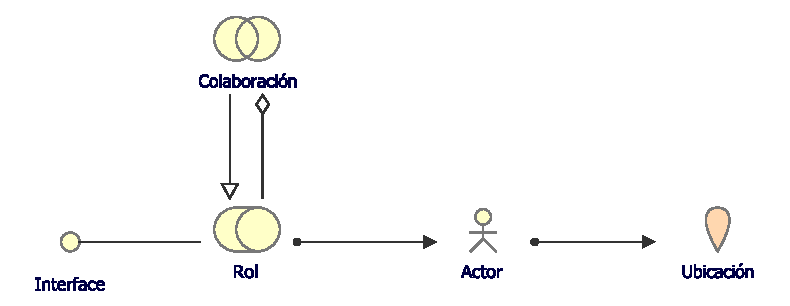
\includegraphics[width=1\linewidth]{ARQUITECTURA/imgs/MOrganizacion}
	\caption{Modelo de Ogranización}
\end{figure}


\newpage
\subsection{Caso de Estudio}

\begin{figure}[h!]
	\centering
	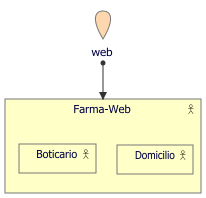
\includegraphics[width=.5\linewidth]{ARQUITECTURA/imgs/COrganizacion}
	\caption{Modelo de Ogranización}
\end{figure}

 Explicacmos nuestro caso de estudio
\newpage
%---------------------------------
\section{Punto de Vista de Coperación de Actor}
\subsection{Modelo}
The Organization viewpoint focuses on the (internal) organization of a company, a department, a network of companies, or of another organizational entity. It is possible to present models in this viewpoint as nested block diagrams, but also in a more traditional way, such as organizational charts. The Organization viewpoint is very useful in identifying competencies, authority, and responsibilities in an

\begin{figure}[h!]
	\centering
	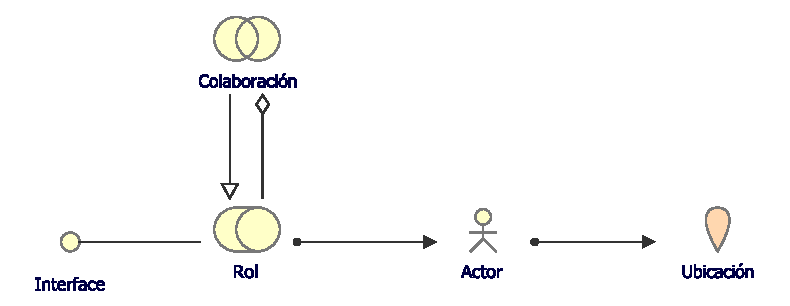
\includegraphics[width=1\linewidth]{ARQUITECTURA/imgs/MOrganizacion}
	\caption{Modelo de Ogranización}
\end{figure}


\newpage
\subsection{Caso de Estudio}

\begin{figure}[h!]
	\centering
	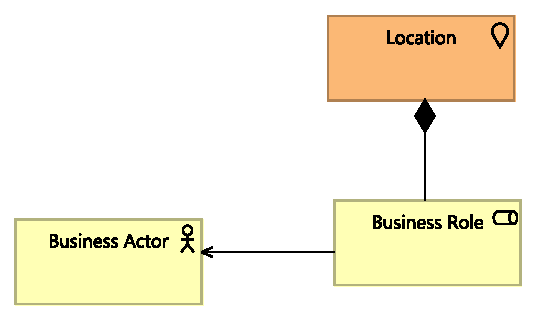
\includegraphics[width=.5\linewidth]{ARQUITECTURA/imgs/COrganizacion1}
	\caption{Modelo de Ogranización}
\end{figure}
Explicacmos nuestro caso de estudio
\newpage
%---------------------------------
\section{Punto de Vista de Fcunión de Negocio}
\subsection{Modelo}
The Organization viewpoint focuses on the (internal) organization of a company, a department, a network of companies, or of another organizational entity. It is possible to present models in this viewpoint as nested block diagrams, but also in a more traditional way, such as organizational charts. The Organization viewpoint is very useful in identifying competencies, authority, and responsibilities in an

\begin{figure}[h!]
	\centering
	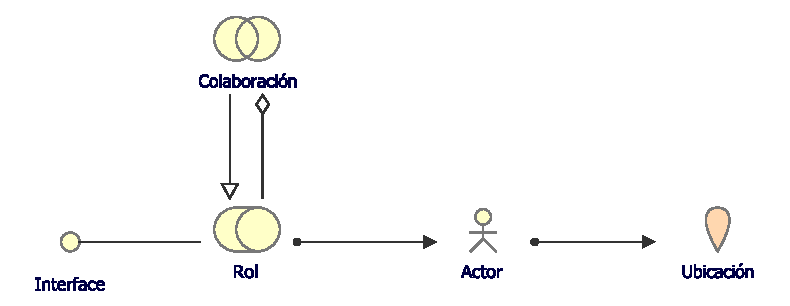
\includegraphics[width=1\linewidth]{ARQUITECTURA/imgs/MOrganizacion}
	\caption{Modelo de Ogranización}
\end{figure}


\newpage
\subsection{Caso de Estudio}

\begin{figure}[h!]
	\centering
	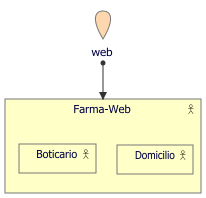
\includegraphics[width=.5\linewidth]{ARQUITECTURA/imgs/COrganizacion}
	\caption{Modelo de Ogranización}
\end{figure}
Explicacmos nuestro caso de estudio
\newpage
%---------------------------------
\section{Punto de Vista de Proceso de Negocio}
\subsection{Modelo}
The Organization viewpoint focuses on the (internal) organization of a company, a department, a network of companies, or of another organizational entity. It is possible to present models in this viewpoint as nested block diagrams, but also in a more traditional way, such as organizational charts. The Organization viewpoint is very useful in identifying competencies, authority, and responsibilities in an

\begin{figure}[h!]
	\centering
	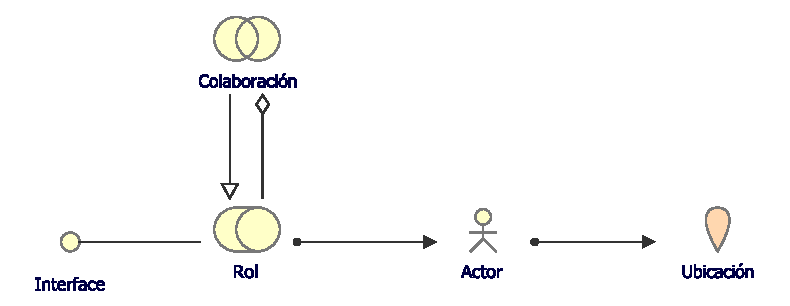
\includegraphics[width=1\linewidth]{ARQUITECTURA/imgs/MOrganizacion}
	\caption{Modelo de Ogranización}
\end{figure}


\newpage
\subsection{Caso de Estudio}

\begin{figure}[h!]
	\centering
	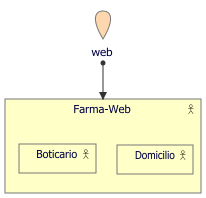
\includegraphics[width=.5\linewidth]{ARQUITECTURA/imgs/COrganizacion}
	\caption{Modelo de Ogranización}
\end{figure}
Explicacmos nuestro caso de estudio
\newpage
%---------------------------------
\section{Punto de Vista de Cooperación de Proceso de Negocio}
\subsection{Modelo}
The Organization viewpoint focuses on the (internal) organization of a company, a department, a network of companies, or of another organizational entity. It is possible to present models in this viewpoint as nested block diagrams, but also in a more traditional way, such as organizational charts. The Organization viewpoint is very useful in identifying competencies, authority, and responsibilities in an

\begin{figure}[h!]
	\centering
	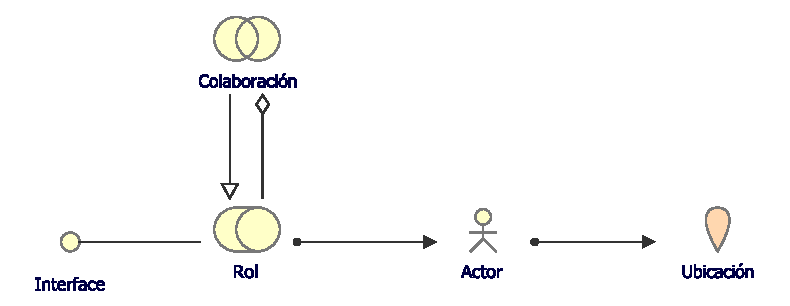
\includegraphics[width=1\linewidth]{ARQUITECTURA/imgs/MOrganizacion}
	\caption{Modelo de Ogranización}
\end{figure}


\newpage
\subsection{Caso de Estudio}

\begin{figure}[h!]
	\centering
	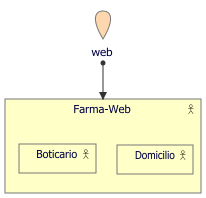
\includegraphics[width=.5\linewidth]{ARQUITECTURA/imgs/COrganizacion}
	\caption{Modelo de Ogranización}
\end{figure}
Explicacmos nuestro caso de estudio
\newpage

%---------------------------------
\section{Punto de Producto}
\subsection{Modelo}
The Organization viewpoint focuses on the (internal) organization of a company, a department, a network of companies, or of another organizational entity. It is possible to present models in this viewpoint as nested block diagrams, but also in a more traditional way, such as organizational charts. The Organization viewpoint is very useful in identifying competencies, authority, and responsibilities in an

\begin{figure}[h!]
	\centering
	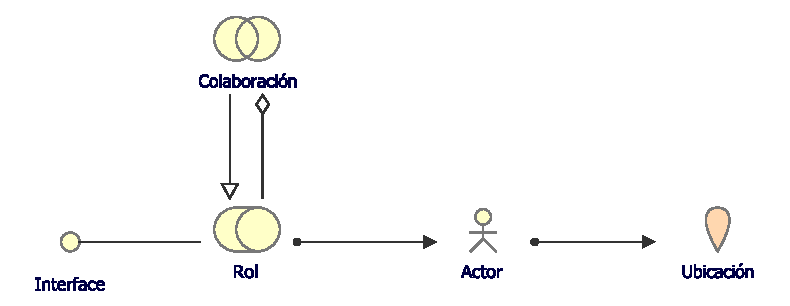
\includegraphics[width=1\linewidth]{ARQUITECTURA/imgs/MOrganizacion}
	\caption{Modelo de Ogranización}
\end{figure}


\newpage
\subsection{Caso de Estudio}

\begin{figure}[h!]
	\centering
	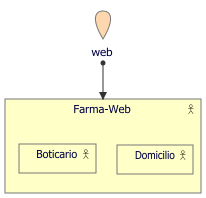
\includegraphics[width=.5\linewidth]{ARQUITECTURA/imgs/COrganizacion}
	\caption{Modelo de Ogranización}
\end{figure}
Explicacmos nuestro caso de estudio
\newpage

\chapter{Capa de Aplicación}
\section{Introducción}
contenido...
\newpage
\chapter{Capa de Tecnología}
\section{Introducción}
contenido...
\newpage
\chapter{Capa de Proyecto}
\section{Introducción}
contenido...
\newpage
\chapter{Capa de Motivación}
\section{Introducción}
contenido...
\newpage
\chapter{Capa de Estartegia}
\section{Introducción}
contenido...
\newpage


\chapter{Patrones GoF}
\section{Introducción}
contenido...
\newpage


\chapter{Patrones Creacionales}
\section{Introducción}
contenido...
\newpage

\section{Singleton}

\subsection{Realización}
\begin{figure}[h!]
	\centering
	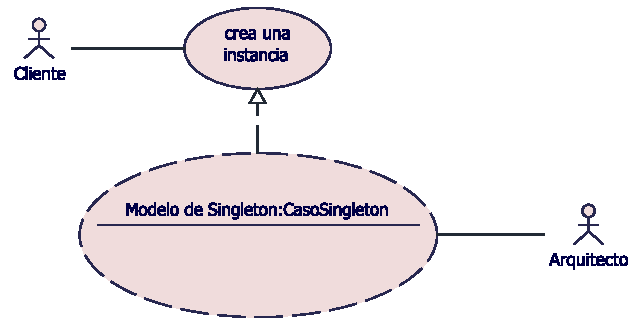
\includegraphics[width=0.7\linewidth]{PATRONES/imgs/MRSingleton}
	\caption{Realizacion de Singleton}
	\label{fig:mrsingleton}
\end{figure}

\subsection{Modelo}
\begin{figure}[h!]
	\centering
	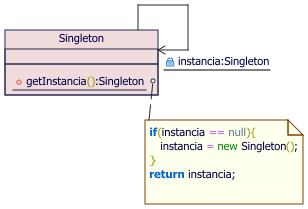
\includegraphics[width=0.7\linewidth]{PATRONES/imgs/MCSingleton}
	\caption{Realizacion de Singleton}
	\label{fig:mrsingleton}
\end{figure}
\subsection{Implementación}
\begin{figure}[h!]
	\centering
	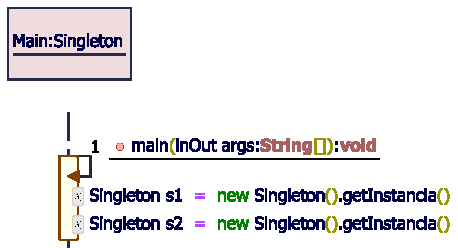
\includegraphics[width=0.7\linewidth]{PATRONES/imgs/MISingleton}
	\caption{Realizacion de Singleton}
	\label{fig:mrsingleton}
\end{figure}
\newpage
\lstinputlisting[caption=Sinlgeton]{c:/a/Singleton.java}

\subsection{Fuentes}
\chapter{Patrones Estructurales}
\section{Introducción}
contenido...
\newpage
\chapter{Patrones de Comportamiento}
\section{Introducción}
contenido...
\newpage


\part{REFLEXIONES}

\bibliographystyle{plain}
\bibliography{REFERENCIA/libros,REFERENCIA/articulos}

\end{document}